\begin{strip}
\centering
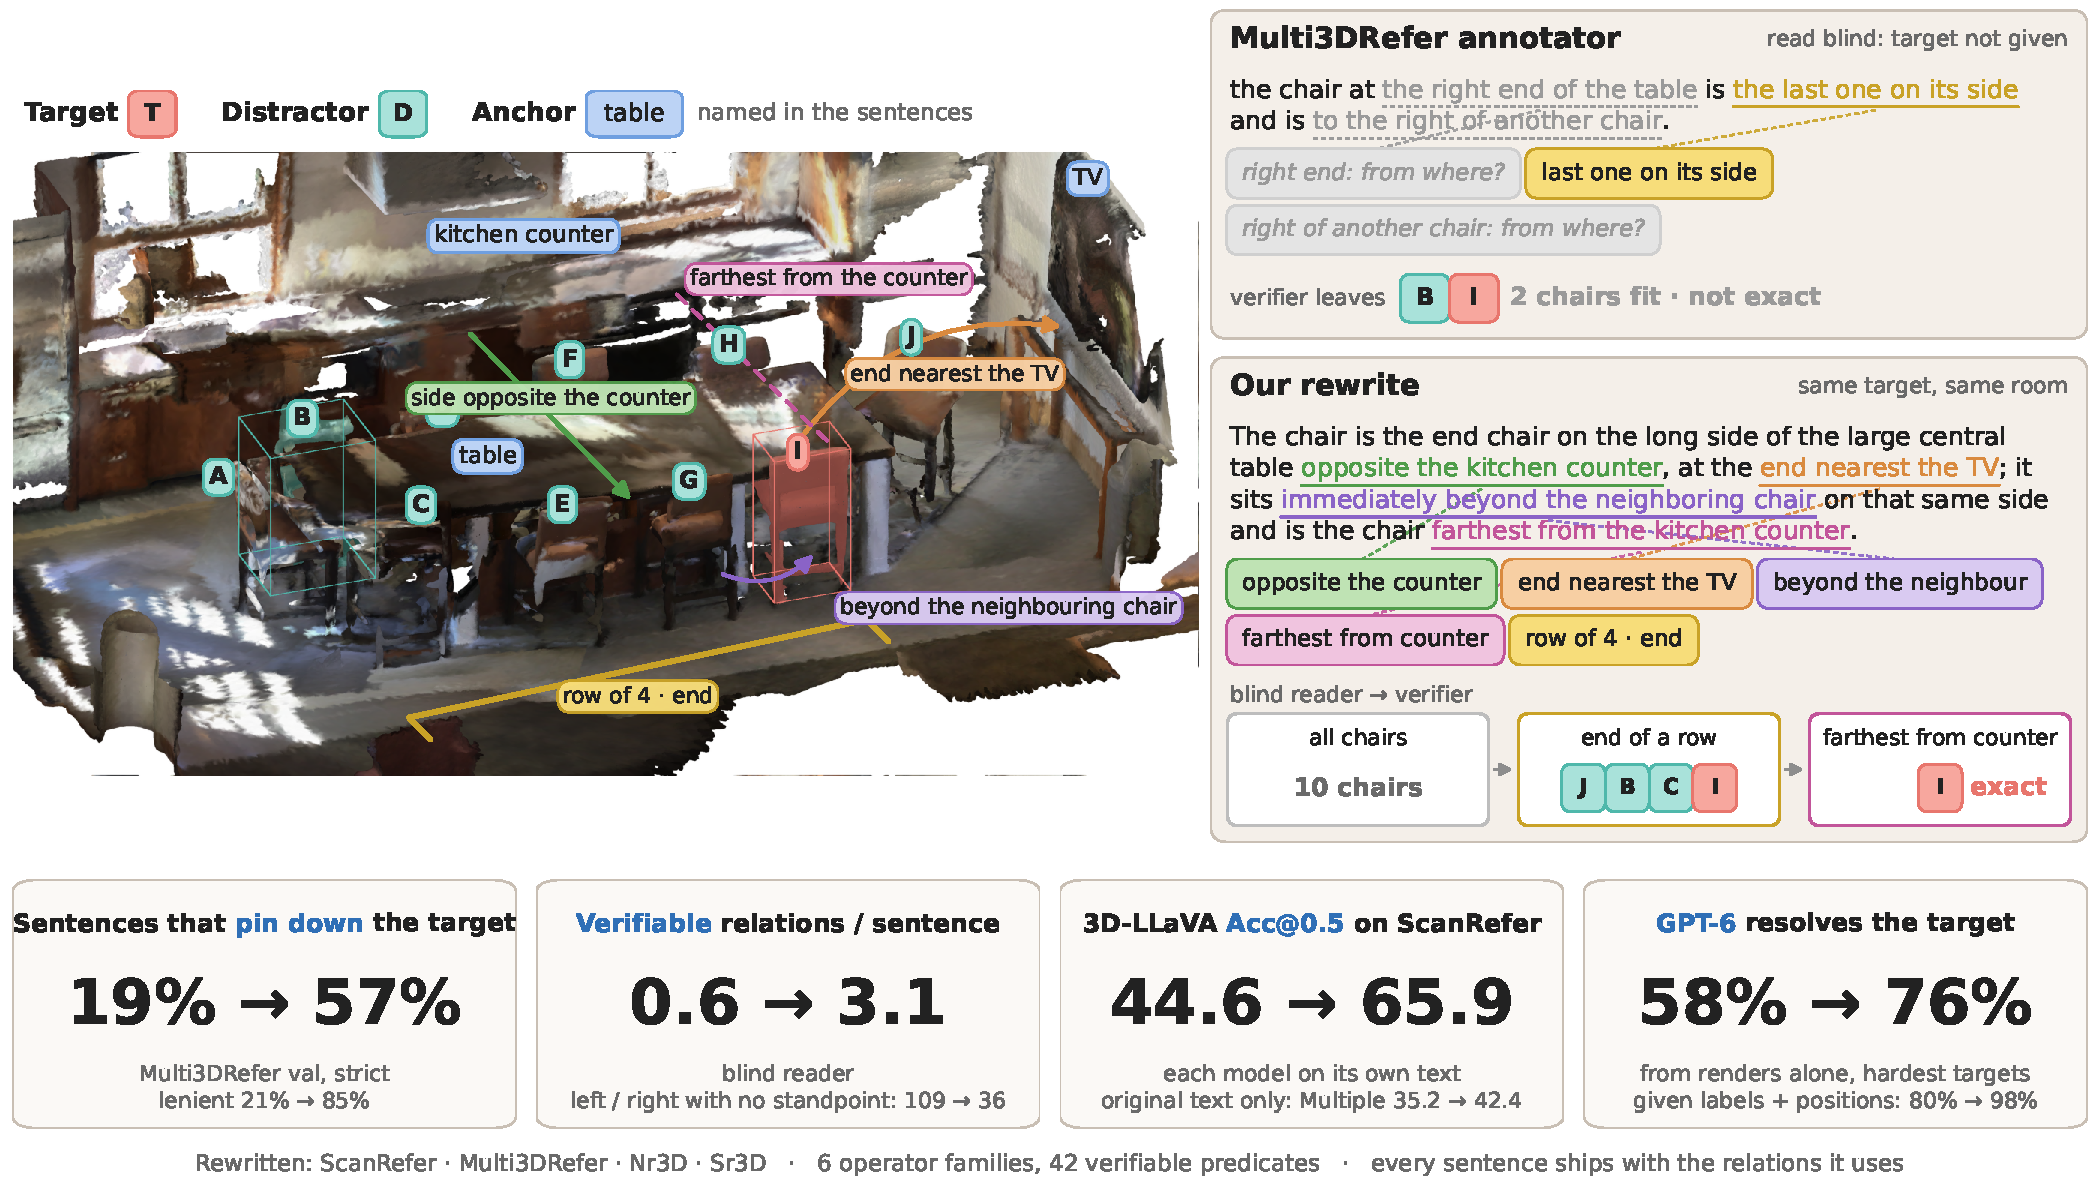
\includegraphics[width=\linewidth]{fig/teaser.pdf}
\captionsetup{hypcap=false}
\captionof{figure}{\textbf{A sentence that does not pin down its target, and the same target rewritten so that it does.}
A Multi3DRefer annotator describes chair~I in a ScanNet dining room (scene0011\_00).
Read blind---without being told the target---the only clause that binds to geometry is \emph{the last one on its side}, and two chairs satisfy it (B and I); \emph{right end} and \emph{right of} name no standpoint (grey).
Our rewrite uses anchors that exist in the room (the kitchen counter, the TV) and relations our operators computed and checked; each clause is coloured like its chip and like the relation drawn on the scene, and the same blind reader and verifier leave one chair.
Tags: target red, same-class candidates teal, anchors named by the sentences blue.
Bottom, left to right: how many sentences pin down their target; how many verifiable relations they carry; what 3D-LLaVA scores when each model is trained and tested on its own text (and, on the original text alone, on targets with same-class distractors); what GPT-6 resolves from the same renders.
\TODO{re-sync the four numbers with the final tables.}}
\captionsetup{hypcap=true}
\label{fig:\currfilebase}%
\end{strip}
